%package list
\documentclass{article}
\usepackage[top=3cm, bottom=3cm, outer=3cm, inner=3cm]{geometry}
\usepackage{multicol}
\usepackage{graphicx}
\usepackage{url}
%\usepackage{cite}
\usepackage{hyperref}
\usepackage{array}
%\usepackage{multicol}
\newcolumntype{x}[1]{>{\centering\arraybackslash\hspace{0pt}}p{#1}}
\usepackage{natbib}
\usepackage{pdfpages}
\usepackage{multirow}
\usepackage[normalem]{ulem}
\useunder{\uline}{\ul}{}
\usepackage{svg}
\usepackage{xcolor}
\usepackage{listings}
\lstdefinestyle{ascii-tree}{
	literate={├}{|}1 {─}{--}1 {└}{+}1 
}
\lstset{basicstyle=\ttfamily,
	showstringspaces=false,
	commentstyle=\color{red},
	keywordstyle=\color{blue}
}
%\usepackage{booktabs}
\usepackage{caption}
\usepackage{subcaption}
\usepackage{float}
\usepackage{array}

\newcolumntype{M}[1]{>{\centering\arraybackslash}m{#1}}
\newcolumntype{N}{@{}m{0pt}@{}}


%%%%%%%%%%%%%%%%%%%%%%%%%%%%%%%%%%%%%%%%%%%%%%%%%%%%%%%%%%%%%%%%%%%%%%%%%%%%
%%%%%%%%%%%%%%%%%%%%%%%%%%%%%%%%%%%%%%%%%%%%%%%%%%%%%%%%%%%%%%%%%%%%%%%%%%%%
\newcommand{\itemEmail}{jchuraaca@unsa.edu.pe}
\newcommand{\itemStudent}{Julio Rubén Chura Acabana}
\newcommand{\itemCourse}{ F. de Programción 2}
\newcommand{\itemCourseCode}{20230472}
\newcommand{\itemSemester}{I}
\newcommand{\itemUniversity}{Universidad Nacional de San Agustín de Arequipa}
\newcommand{\itemFaculty}{Facultad de Ingeniería de Producción y Servicios}
\newcommand{\itemDepartment}{Departamento Académico de Ingeniería de Sistemas e Informática}
\newcommand{\itemSchool}{Escuela Profesional de Ingeniería de Sistemas}
\newcommand{\itemAcademic}{2023 - B}
\newcommand{\itemInput}{Del 11 Septiembre 2023}
\newcommand{\itemOutput}{Al 13 Septiembre 2023}
\newcommand{\itemPracticeNumber}{01}
\newcommand{\itemTheme}{Arreglos Estandar}
%%%%%%%%%%%%%%%%%%%%%%%%%%%%%%%%%%%%%%%%%%%%%%%%%%%%%%%%%%%%%%%%%%%%%%%%%%%%
%%%%%%%%%%%%%%%%%%%%%%%%%%%%%%%%%%%%%%%%%%%%%%%%%%%%%%%%%%%%%%%%%%%%%%%%%%%%

\usepackage[english,spanish]{babel}
\usepackage[utf8]{inputenc}
\AtBeginDocument{\selectlanguage{spanish}}
\renewcommand{\figurename}{Figura}
\renewcommand{\refname}{Referencias}
\renewcommand{\tablename}{Tabla} %esto no funciona cuando se usa babel
\AtBeginDocument{%
	\renewcommand\tablename{Tabla}
}

\usepackage{fancyhdr}
\pagestyle{fancy}
\fancyhf{}
\setlength{\headheight}{30pt}
\renewcommand{\headrulewidth}{1pt}
\renewcommand{\footrulewidth}{1pt}
\fancyhead[L]{\raisebox{-0.2\height}{
\includegraphics[width=3cm]{img/logo_episunsa.png}}}
\fancyhead[C]{\fontsize{7}{7}\selectfont	\itemUniversity \\ \itemFaculty \\ \itemDepartment \\ \itemSchool \\ \textbf{\itemCourse}}
\fancyhead[R]{\raisebox{-0.2\height}{
\includegraphics[width=1.2cm]{img/logo_abet}}}
\fancyfoot[L]{Estudiante Julio Rubén Chura Acabana}
\fancyfoot[C]{\itemCourse}
\fancyfoot[R]{Página \thepage}

% para el codigo fuente
\usepackage{listings}
\usepackage{color, colortbl}
\definecolor{dkgreen}{rgb}{0,0.6,0}
\definecolor{gray}{rgb}{0.5,0.5,0.5}
\definecolor{mauve}{rgb}{0.58,0,0.82}
\definecolor{codebackground}{rgb}{0.95, 0.95, 0.92}
\definecolor{tablebackground}{rgb}{0.8, 0, 0}

\lstset{frame=tb,
	language=bash,
	aboveskip=3mm,
	belowskip=3mm,
	showstringspaces=false,
	columns=flexible,
	basicstyle={\small\ttfamily},
	numbers=none,
	numberstyle=\tiny\color{gray},
	keywordstyle=\color{blue},
	commentstyle=\color{dkgreen},
	stringstyle=\color{mauve},
	breaklines=true,
	breakatwhitespace=true,
	tabsize=3,
	backgroundcolor= \color{codebackground},
}

\begin{document}
	
	\vspace*{10px}
	
	\begin{center}	
		\fontsize{17}{17} \textbf{ Informe de Laboratorio \itemPracticeNumber}
	\end{center}
	\centerline{\textbf{\Large Tema: \itemTheme}}
	%\vspace*{0.5cm}	
	
	\begin{flushright}
		\begin{tabular}{|M{2.5cm}|N|}
			\hline 
			\rowcolor{tablebackground}
			\color{white} \textbf{Nota}  \\
			\hline 
			\\[30pt]
			\hline 			
		\end{tabular}
	\end{flushright}	
	
	\begin{table}[H]
		\begin{tabular}{|x{4.7cm}|x{4.8cm}|x{4.8cm}|}
			\hline 
			\rowcolor{tablebackground}
			\color{white} \textbf{Estudiante} & \color{white}\textbf{Escuela}  & \color{white}\textbf{Asignatura}   \\
			\hline 
			{\itemStudent \par \itemEmail} & \itemSchool & {\itemCourse \par Semestre: \itemSemester \par Código: \itemCourseCode}     \\
			\hline 			
		\end{tabular}
	\end{table}		
	
	\begin{table}[H]
		\begin{tabular}{|x{4.7cm}|x{4.8cm}|x{4.8cm}|}
			\hline 
			\rowcolor{tablebackground}
			\color{white}\textbf{Laboratorio} & \color{white}\textbf{Tema}  & \color{white}\textbf{Duración}   \\
			\hline 
			\itemPracticeNumber & \itemTheme & 04 horas   \\
			\hline 
		\end{tabular}
	\end{table}
	
	\begin{table}[H]
		\begin{tabular}{|x{4.7cm}|x{4.8cm}|x{4.8cm}|}
			\hline 
			\rowcolor{tablebackground}
			\color{white}\textbf{Semestre académico} & \color{white}\textbf{Fecha de inicio}  & \color{white}\textbf{Fecha de entrega}   \\
			\hline 
			\itemAcademic & \itemInput &  \itemOutput  \\
			\hline 
		\end{tabular}
	\end{table}
	
	\section{Tarea}
	\begin{itemize}		
		\item Escribir un código donde se creen 5 soldados considerando su nombre usando variables simples
		\item Crear 5 soldados con sus respectivos nombres y nivel de vida usando variables simples
		\item Crear 5 soldados considerando su nombre usando arreglos estandar.
		\item Crear 5 soldados considerando su nombre y nivel de vida usando arreglos
		\item Crear dos arreglos de soldados y determinar quien gana considerando como condición de victoria el bando que tenga mayor cantidad de soldados
		\item Trabajar los 5 ejercicios en un mismo archivo pero se deberá subir al repositorio cada versión. Luego se presentará un informe de la sesión
	\end{itemize}
	
	\section{Equipos, materiales y temas utilizados}
	\begin{itemize}
		\item Sistema Operativo Windows
		\item VIM 9.0.
		\item OpenJDK 64-Bits 17.0.7.
		\item Git 2.39.2.
		\item Cuenta en GitHub con el correo institucional.
		\item Arreglos Estándar
	\end{itemize}
	
	\section{URL de Repositorio Github}
	\begin{itemize}
		\item URL del Repositorio GitHub para clonar o recuperar.
		\item \url{https://github.com/JulioChura/fp2-23b.git}
		\item URL para el laboratorio 01 en el Repositorio GitHub.
		\item \url{https://github.com/JulioChura/fp2-23b/tree/main/fase01/lab01}
	\end{itemize}
	
	\section{Actividades con el repositorio GitHub}
	
	\subsection{Creando e inicializando repositorio GitHub}
	\begin{itemize}	
		\item Como es el primer laboratorio se creo el repositorio GitHub.
		\item Se realizaron los siguientes comandos en la computadora:
	\end{itemize}	
	
	\begin{lstlisting}[language=bash,caption={Creando directorio de trabajo}][H]
		mkdir fp2-23b\fase01\lab01
		cd fp2-23b
		mkdir fase02
		mkdir fase03
		
	\end{lstlisting}
	\begin{lstlisting}[language=bash,caption={Dirijíéndonos al directorio de trabajo}][H]
		cd fp2-23b
	\end{lstlisting}	
	
	\begin{lstlisting}[language=bash,caption={Inicializando directorio para repositorio GitHub}][H]
		cd C:\Users\USUARIO\Desktop\fp2-23b
		git init
		git config --global user.name "Julio Chura"
		git config --global user.email jchuraaca@unsa.edu.pe
		git add README.md
		git commit -m "Se agrega el proyecto"
		git branch -M main
		git remote add origin https://github.com/JulioChura/fp2-23b.git
		git push -u origin main
	\end{lstlisting}
	
	\subsection{Commits}
	\begin{lstlisting}[language=bash,caption={Primer Commit Creando carpeta/archivo para laboratorio 01}][H]
		cd fase01/lab01
		vim VideoJuego.java
		git add .
		git commit -m "Creando el archivo VideoJuego.java"			
		$ git push -u origin main
	\end{lstlisting}
	
	\begin{itemize}	
		\item Se creo el archivo \textbf{.gitignore} para no considerar los archivos \textbf{*.class} que son innecesarios hacer seguimiento.
	\end{itemize}
	\begin{lstlisting}[language=bash,caption={Creando .gitignore}][H]
		cd C:\Users\USUARIO\Desktop\fp2-23b
		vim .gitignore
	\end{lstlisting}
	\begin{lstlisting}[language=bash,caption={lab01/.gitignore}][H]
		*.class
	\end{lstlisting}
	\begin{lstlisting}[language=bash,caption={Commit: Creando .gitignore para archivos *.class y creando VideoJuego.java}][H]
		git add .
		git commit -m "Subiendo gitignore"			
		git push -u origin main
		cd fp2-23b\fase01\lab01
		vim VideoJuego.java
	\end{lstlisting}
	
	\begin{itemize}	
		\item Para el siguiente commit, se resuelve el primer y segundo ejercicio de la práctica, el cual consiste en crear 5 soldados con su respectivo nombre y con su nivel de vida, para ello se hace uso de variables simples como se indica
		\item En esta parte, por lo general las líneas 12, 13, 14, 15  del código se repetirán de forma constante teniendo pequeñas variaciones. Más antes de esta versión se realizó otra pero ingresando solo los nombres de los soldados, debido a que esta versión abarca la primera parte se optó por considerar esta
	\end{itemize}	
	
	\begin{figure}[H]
		\centering
		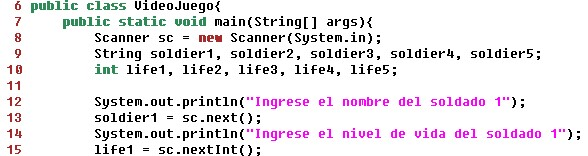
\includegraphics[width=0.8\textwidth,keepaspectratio]{img/fragmento_codigoPartel.jpg}
		%\includesvg{img/automata.svg}
		%\label{img:mot2}
		%\caption{Product backlog.}
	\end{figure}
	
	\clearpage
	
	\begin{lstlisting}[language=bash,caption={Subiendo al repositorio los cambios realizados al código VideoJuego.java}][H]
		git add VideoJuego.java
		git commit -"Poner nivel de vida de cada soldado y mostrarlo"
		git push -u origin main
	\end{lstlisting}
	
	\begin{lstlisting}[language=bash,caption={Uso de  arreglos y números aleatorios para crear los soldados y su vida}][H]
		vim VideoJuego.java
	\end{lstlisting}
	
	\begin{figure}[H]
		\centering
		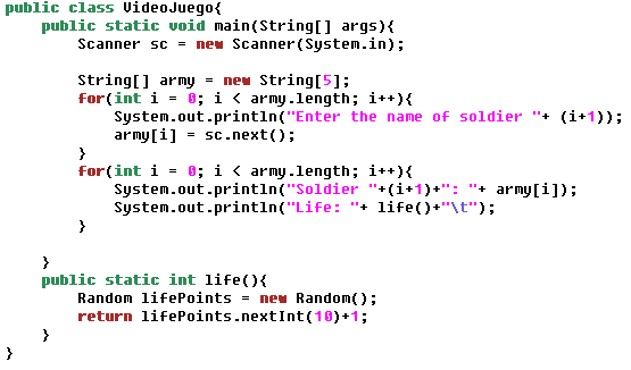
\includegraphics[width=0.8\textwidth,keepaspectratio]{img/fragmento_codigoPartell.jpg}
		%\includesvg{img/automata.svg}
		%\label{img:mot2}
		%\caption{Product backlog.}
	\end{figure}
	
	\begin{lstlisting}[language=bash,caption={Subiendo los cambios al repositorio}][H]
		git add VideoJuego.java
		git commit -m "Anadiendo la vida de cada soldado usando numeros aleatorios"
	\end{lstlisting}
	
	\begin{lstlisting}[language=bash,caption={Ejercicio 5: Enfrentamiento entre dos ejercitos}]	
		vim VideoJuego.java
	\end{lstlisting}
	
	\lstinputlisting[language=Java, caption={VideoJuego.java terminado},numbers=left,]{src/VideoJuego.java}
	
	\begin{lstlisting}[language=bash,caption={Compilando y probando código}][H]
		javac VideoJuego.java
		java VideoJuego
		ARMY 1
		Soldier1
		Soldier2
		Soldier3
		
		ARMY 2
		Soldier1
		
		The winner is the army 1
	\end{lstlisting}
	
	\begin{lstlisting}[language=bash,caption={Commit: Subiendo al repositorio la versión final del ejercicio }][H]
		$ git add .
		$ git commit -m "Eliminando lineas inncesarias"			
		$ git push -u origin main
	\end{lstlisting}
	
	
	\subsection{Estructura de laboratorio 01}
	\begin{itemize}	
		\item El contenido que se entrega en este laboratorio es el siguiente:
	\end{itemize}
	
	\begin{lstlisting}[style=ascii-tree]
		lab01/
		|--- VideoJuego.java
		|--- latex
		|--- img
		|   |--- logo_abet.png
		|   |--- logo_episunsa.png
		|   |--- logo_unsa.jpg
		|   |--- fragmento_codigoPartel.jpg    
		|   |--- fragmento_codigoPartell.jpg
		|--- programacion_lab01_rescobedoq_v1.0.pdf    
		|--- programacion_lab01_rescobedoq_v1.0.tex
		|--- src
		|	 |--- VideoJuego.java
	\end{lstlisting}    
	
	\section{\textcolor{red}{Rúbricas}}
	
	\subsection{\textcolor{red}{Entregable Informe}}
	\begin{table}[H]
		\caption{Tipo de Informe}
		\setlength{\tabcolsep}{0.5em} % for the horizontal padding
		{\renewcommand{\arraystretch}{1.5}% for the vertical padding
			\begin{tabular}{|p{3cm}|p{12cm}|}
				\hline
				\multicolumn{2}{|c|}{\textbf{\textcolor{red}{Informe}}}  \\
				\hline 
				\textbf{\textcolor{red}{Latex}} & \textcolor{blue}{El informe está en formato PDF desde Latex,  con un formato limpio (buena presentación) y facil de leer.}   \\ 
				\hline 
				
				
			\end{tabular}
		}
	\end{table}
	
	\clearpage
	
	\subsection{\textcolor{red}{Rúbrica para el contenido del Informe y demostración}}
	\begin{itemize}			
		\item El alumno debe marcar o dejar en blanco en celdas de la columna \textbf{Checklist} si cumplio con el ítem correspondiente.
		\item Si un alumno supera la fecha de entrega,  su calificación será sobre la nota mínima aprobada, siempre y cuando cumpla con todos lo items.
		\item El alumno debe autocalificarse en la columna \textbf{Estudiante} de acuerdo a la siguiente tabla:
		
		\begin{table}[ht]
			\caption{Niveles de desempeño}
			\begin{center}
				\begin{tabular}{ccccc}
					\hline
					& \multicolumn{4}{c}{Nivel}\\
					\cline{1-5}
					\textbf{Puntos} & Insatisfactorio 25\%& En Proceso 50\% & Satisfactorio 75\% & Sobresaliente 100\%\\
					\textbf{2.0}&0.5&1.0&1.5&2.0\\
					\textbf{4.0}&1.0&2.0&3.0&4.0\\
					\hline
				\end{tabular}
			\end{center}
		\end{table}	
		
	\end{itemize}
	
	\begin{table}[H]
		\caption{Rúbrica para contenido del Informe y demostración}
		\setlength{\tabcolsep}{0.5em} % for the horizontal padding
		{\renewcommand{\arraystretch}{1.5}% for the vertical padding
			%\begin{center}
			\begin{tabular}{|p{2.7cm}|p{7cm}|x{1.3cm}|p{1.2cm}|p{1.5cm}|p{1.1cm}|}
				\hline
				\multicolumn{2}{|c|}{Contenido y demostración} & Puntos & Checklist & Estudiante & Profesor\\
				\hline
				\textbf{1. GitHub} & Hay enlace URL activo del directorio para el  laboratorio hacia su repositorio GitHub con código fuente terminado y fácil de revisar. &2 &X &2 & \\ 
				\hline
				\textbf{2. Commits} &  Hay capturas de pantalla de los commits más importantes con sus explicaciones detalladas. (El profesor puede preguntar para refrendar calificación). &4 &X &2 & \\ 
				\hline 
				\textbf{3. Código fuente} &  Hay porciones de código fuente importantes con numeración y explicaciones detalladas de sus funciones. &2 &X &2 & \\ 
				\hline 
				\textbf{4. Ejecución} & Se incluyen ejecuciones/pruebas del código fuente  explicadas gradualmente. &2 &X &1 & \\ 
				\hline			
				\textbf{5. Pregunta} & Se responde con completitud a la pregunta formulada en la tarea.  (El profesor puede preguntar para refrendar calificación).  &2 &X &2 & \\ 
				\hline	
				\textbf{6. Fechas} & Las fechas de modificación del código fuente estan dentro de los plazos de fecha de entrega establecidos. &2 &X &2 & \\ 
				\hline 
				\textbf{7. Ortografía} & El documento no muestra errores ortográficos. &2 &X &2 & \\ 
				\hline 
				\textbf{8. Madurez} & El Informe muestra de manera general una evolución de la madurez del código fuente,  explicaciones puntuales pero precisas y un acabado impecable.   (El profesor puede preguntar para refrendar calificación).  &4 &X &2 & \\ 
				\hline
				\multicolumn{2}{|c|}{\textbf{Total}} &20 & &15 & \\ 
				\hline
			\end{tabular}
			%\end{center}
			%\label{tab:multicol}
		}
	\end{table}
	
	\clearpage
	
	\section{Referencias}
	\begin{itemize}			
		\item \url{https://drive.google.com/file/d/1MdWf_3UA_38xs18HmjPk6eH0RzRMJxkX/view?usp=drive_link}
		\item \url{https://drive.google.com/file/d/17xNjwcFykmT8BB5VbZrYEDWUg3UjLlRs/view?usp=drive_link}
	\end{itemize}	
	
	%\clearpage
	%\bibliographystyle{apalike}
	%\bibliographystyle{IEEEtranN}
	%\bibliography{bibliography}
	
\end{document}